\documentclass[11pt]{article}
\usepackage[letterpaper,hmargin=0.85in,vmargin=0.7in]{geometry}
\usepackage[T1]{fontenc}
\usepackage[charter,cal=cmcal]{mathdesign}
\usepackage{microtype}
\usepackage{amsmath}
\usepackage{graphicx}
\usepackage{booktabs}
\usepackage[numbers,sort]{natbib}
\usepackage[hidelinks]{hyperref}
\usepackage{url}
\usepackage{enumitem}
\usepackage[compact]{titlesec}
\usepackage{caption}
\captionsetup{font=small,labelfont=bf,skip=3pt}
\titleformat{\section}{\large\bfseries}{\thesection}{0.6em}{}
\titlespacing*{\section}{0pt}{1.1ex plus .3ex}{0.4ex}
\titleformat{\subsection}{\normalsize\bfseries}{\thesubsection}{0.6em}{}
\titlespacing*{\subsection}{0pt}{1.0ex plus .2ex}{0.3ex}
\setlength{\bibsep}{0pt plus .3pt}
\renewcommand{\bibfont}{\footnotesize}
\setlength{\textfloatsep}{7pt plus 2pt}
\setlength{\floatsep}{6pt plus 2pt}
\setlength{\parskip}{0pt}
\setlist{nosep,leftmargin=1.4em}
\newcommand{\code}[1]{\texttt{\small #1}}

% ---- NUMBERS FOR THE CURRENT BOT: the only place the text holds them. -------------------------
% A refresh pass edits these macros, the last row of BOUND_ROWS in figures/make_figs.py, and the
% sentences tagged SERVED-PROSE below. All of them are listed in board/rb-track/story-numbers.md.
% DATING RULE: stages are named (the original bot, the told-type policy, the first hidden-hand
% policy, the current bot); no clock times or day-level dates in prose, figures or captions.
\newcommand{\servedbound}{0.1525}      % eps_G, sum of both seats (served-now.json epsSum)
\newcommand{\servedboundshort}{0.15}   % the same, two decimals
\newcommand{\servedwin}{53.9\%}        % 50% + bound/4, rounded up
\newcommand{\servedvlo}{-0.058}        % v_lo (served-now.json vLo)
\newcommand{\servedvhi}{+0.094}        % v_hi (served-now.json vHi)
\newcommand{\servedprobe}{0.088}       % probe on the current bot (interim)
\newcommand{\servedprobese}{0.050}
\newcommand{\servedprobepairs}{750 pairs into a run of 1,000}
% ----------------------------------------------------------------------------------------------

% Sources. Every number below is in board/claims.md (entries named in brackets), in
% board/rb-track/bound-ledger.md (ledger:), in board/rb-track/served-now.json, or in the Red/Black
% manuscripts (rb:) as named here. Figures: report/figures/make_figs.py.
%  hand: games/redblack/README.md, generate.py KNOWN (rb-pennies -1/2, 1,551 nodes; leaky 0, 150 pairs);
%        15.5%: rb Paper II and its solver notes (the first solver's leak; 15.5%).
%  arc:  four manuscripts, rb:research/README.md; 2.4e33 infosets, Paper I; lower bound only,
%        Paper III Remark "Paused, with a lower bound only".
%  core: [js-demo] 1,245 lines; [redteam-fix] 103 obligations, 281/281 pairs over 61 games;
%        random games 20,000 + 2,577 (story-factcheck.md).
%  agents: experiment/RESULTS.md, [experiment-run] (6 models, 5 cells, 4 replicates = 120).
%  guards: [report-v2] P3/numbers.json; deck/assets/rb_before_after.json (72 of 132 above 0.1 with the
%        original guards; d0-3.2.1-1.0.1 0.1286 original, 0.0045 fixed; book median 1.3e-5, max 3.05e-4).
%  probe on the original bot: ledger "Probe lower bounds" (win rate 0.7970, eps_G 1.1880 SE 0.0201;
%        3,000 mirrored pairs = 6,000 games).
%  ceilings: ledger "Upper bounds": 0.6992, 0.3021, 0.2522, 0.2197, 0.1953, 0.1525; a later pass 0.1432.
%        Win-rate reading: 50% + eps_G/4 over a seat-swapped pair (payoffs +1 / -1), rounded up.
%  checks on the current bot's store: served-now.json "checks".
%  probe on the later stages: ledger "Probe lower bounds" (0.2632 SE 0.0192; 0.2407 SE 0.0249 against
%        0.2373 on the same 3,000 deals, paired +0.0033 SE 0.0331; 0.2560 SE 0.0429).
%  coins: ledger "Caveats" FIXED row (103/103 mixed decisions on 7 games, chance 56.5; after: 21/32,
%        chance 18.3).
%  gap: about three quarters of the charge is real on small classes (solver notes, next steps).

\title{\vspace{-2.2em}\Large\textbf{Call the Bluff: Grading Game Strategies with a Verified Checker}}
\author{Noah Brauner\\\small CS 2520r, Harvard University, November 2026}
\date{}

\begin{document}
\maketitle
\vspace{-2.1em}

{\small\noindent\textbf{Abstract.} A game solver that reports convergence is grading itself against its own model of the
game, which may be wrong. I describe a checker that grades the strategy instead. Given a finite two-player
zero-sum game and a strategy for each player, it computes both best-response values in exact
rational arithmetic, and its 1,245-line Dafny core proves that no strategy does better than the
value it reports. In 144 runs of mutant and reference CFR solvers, 19 declared convergence while exploitable
by at least $0.01$. Of 93 convergence claims from solvers that six Claude models wrote, 13 were
false. In my bot for the bidding game Red/Black, the checker found a pruning rule that
raised median exploitability on 132 endgames from $0.019$ to $0.129$. The full game is too large to
enumerate, so the current bot has a floating-point ceiling instead: no opponent can expect to
win more than $\servedwin$ of a seat-swapped pair of games.
\par}

\section{Introduction}

A strategy for a game of hidden information can be wrong in a way nobody sees by playing it. The
usual evidence that it is good is the solver's own report that it converged, which means that some
quantity it computes from its model of the game has stopped moving. A solver with the wrong model of the game converges
just as happily, to an equilibrium of the wrong game.

I ran into this while building solvers for Red/Black, a bidding game I designed and run at
\href{https://www.playredblack.com}{playredblack.com}, over the spring and summer of 2026
\cite{rb0,rb1,rb2,rb3}. My very first solver was solving a slightly different game, one where card
identities leaked which card a player threw away. A position I can value by hand at $25\%$
(Section~\ref{sec:guards}) is worth $50\%$ in that game, and every check the solver ran passed,
because every check shared the same wrong rules. I caught it only because I designed the game and
knew a discard is supposed to be private. % NOAH-CONFIRM (source: rb docs/solver/lessons.md #1)
The next version priced the same position at $15.5\%$, which is also wrong, and its own
best-response brackets agreed with it \cite{rb2}.

My approach is to leave the solver unverified and grade its strategy with a checker whose answer
comes with a proof. The first contribution is \code{bin/bluff}, a best-response checker for finite
two-player zero-sum games whose Dafny core is proved correct over exact rationals
(Section~\ref{sec:checker}).\footnote{Code and data: \url{https://github.com/SwiftlyNoah/call-the-bluff}}
The second is two measurements of how often a claim of convergence is false, on mutant CFR solvers
(Section~\ref{sec:mutants}) and on solvers written by AI agents (Section~\ref{sec:agents}). The
third is a case study on my own bot, where a pruning rule I had described as harmless stopped the
bot from bluffing in the positions where it should (Section~\ref{sec:guards}). The full game is far
too big for a checker to read, so for it I give a floating-point ceiling on what any opponent can
win from the bot on the site (Section~\ref{sec:whole}).

\section{Background and related work}

\textbf{Cheap talk.} In an essay earlier this term I called reports like ``all tests pass'' cheap
talk \cite{essay,crawford1982}: they cost the same to send whether or not they are true, so they
carry no information. A convergence meter that shares the solver's
assumptions is cheap talk in the same sense.

\textbf{CFR and exploitability.} The solvers in this paper are variants of counterfactual regret
minimization (CFR) \cite{zinkevich2007} and CFR+ \cite{tammelin2014}. A two-player zero-sum
strategy pair has a measure that does not depend on how it was found, its \emph{exploitability}. Fix both players'
strategies, let each player in turn switch to the best possible reply against the other, and
average how much they gain. It is zero exactly at an equilibrium, and it is how much an opponent who knows your strategy can take from you. The checker reports this
average. My Red/Black papers add the two gains instead, and I write $\varepsilon_G$ for that sum,
which is twice the average and runs from 0 to 2 when a win pays $+1$ and a loss $-1$. Over two
games with the seats swapped, an opponent who gains $\varepsilon_G$ in total wins
$50\%+\varepsilon_G/4$ of them. A best response is itself computed by a program, though,
and a buggy one could report zero for anything.

\textbf{Exploiter probes.} When a game is too large for an exact best response, the usual
substitute is a \emph{probe}, a program that is handed the bot's strategy, keeps a running belief
about the bot's cards, and plays a greedy best reply at every move \cite{lisy2017}. A probe proves
nothing about the worst case, since a better exploiter might take more, but what it takes is a
floor.

\textbf{Verified software and specifications.} Dafny \cite{leino2010} is a programming language
whose compiler checks proofs about the program with an SMT solver. Henniger, Chong and Amin
propose a division of labor for Djinnlang \cite{henniger2026} that I follow here: the human's job
is to state unambiguously what they want, and the machine's job is everything that can be checked
against that statement. In this paper the statement is a game file, and it only partly records the rules in my head, which
is Naur's point about programs in general \cite{naur1985}.

\section{The checker}\label{sec:checker}

The checker, \code{bin/bluff}, reads a game file (a finite tree of chance, decision and terminal
nodes, with every probability and payoff an exact fraction) and a strategy for each player, and
prints both players' best-response values and the exploitability. Its core is 1,245 lines of Dafny
that compute over exact rationals and prove a theorem about whatever they return. If the check
succeeds, no strategy of either player, pure or mixed at each decision, does better against
the other player than the reported best-response value. The pure strategy the checker returns
achieves that value, and the exploitability is half the sum of the two. The proof has 103
obligations, uses no axioms or assumptions, and an audit script refuses to build if anyone adds
one.

One step is checked at run time instead of proved: the returned strategy must pick the same action
everywhere a player cannot tell positions apart, and the checker refuses the game if it does not.
Perfect recall guarantees this, but I did not prove that implication; on about 23,000 random
perfect-recall games it never refused one. The trusted base is everything outside the proof: the
JSON adapter, Dafny 4.11.0, Z3, the compiler, Python, and the game files. On 281 game and strategy
pairs over 61 game files the checker agrees exactly with an independent best response in Python,
and it reproduces Kuhn poker's value of $-1/18$ \cite{kuhn1950}.

The checker grades a strategy no matter who wrote the solver, so I do not have to verify my
own solver or one written by an AI agent. The proof does not cover whether
the game file is the game I meant. Section~\ref{sec:guards} gives an example of a wrong file that the checker certifies.

\section{Evaluation}

\subsection{Mutant solvers}\label{sec:mutants}

I made eleven
one-edit mutants of a correct CFR+ solver and ran them, with clean CFR and CFR+ and three
vanilla-CFR variants, on nine games. In 19 of those 144 runs the solver stopped and declared
convergence while its strategy was exploitable by at least $0.01$. Every one of those had a wrong
model of the game or wrote out a different strategy from the one it measured. An update bug, like
a missing probability weight, never fooled the meter, which measures the strategy the update produces.

\subsection{Solvers written by AI agents}\label{sec:agents}

I asked six Claude models to write CFR solvers for Kuhn poker, Leduc hold'em \cite{southey2005}
and a small Red/Black, 120 trials of up to 30 minutes (six models, five settings, four replicates
each), and had each one end by saying whether its
solver converged. Then the checker graded every strategy. Of 93 claims of convergence, 13 were
false ($14\%$, Wilson 95\% interval $8$ to $22\%$), and 12 of those came from the two older models.
The plainest was a Haiku 4.5 solver for Leduc whose last word was that the game value ``remained
stable at 10.06666667 across 20,000 iterations''. The checker agrees that the solver's strategies give player 0 that value. Leduc is worth about
$-0.09$ to player 0. The value was stable because the
solver's player 1 was maximizing player 0's payoff, and the strategy's exploitability is $6.89$. The newer four
models made 74 claims and got one wrong; Opus 5.5 and Fable 5.2 were right in all 40 of their
trials. The one wrong claim came from a careful Sonnet 5.5 trial that reported exploitability
$0.00609$ from what it called ``an exact best-response calculation''; the certificate says
$0.0860$, fourteen times larger. Its best-response code improved one decision at a time, which
finds a good reply but not always the best.

\subsection{A pruning rule in the live bot}\label{sec:guards}

Red/Black is easiest to explain from the end of a game. I hold one card, and everyone knows it is
red. You hold two, and everyone knows one is red and one is black. The only secret at the table is
the order of your two cards, which you chose. It is my bid. Bids are claims about the cards in
play, and a challenged bidder has to prove the claim by flipping cards off the tops of the
players' piles, losing on the first card of the wrong color. So if I bid ``two red'' and you
challenge, I flip my red and then your top card, and I win only if you put your red on top. If I
bid ``one black'', I win only if you put your black on top. The bidding has a few more branches,
but they all come down to this: I am guessing which card you put on top, and you are hiding it.
That is matching pennies, and the best either of us can do is win half the time. If I lose I am
out. If I win, you must throw away one of your two cards without showing which, and the next round
is the same coin flip over which one you kept. I win this hand with probability exactly
$\tfrac12\cdot\tfrac12=\tfrac14$.

I wrote this hand as a game file twice, once under the real rules and once with the discard leak
of my first solver. The checker certifies an equilibrium of each at exploitability exactly zero,
with values of $25\%$ and $50\%$, since each is a consistent game. A differential test that walks the file in lockstep with the real game engine told them apart. It
found 150 pairs of positions the leaky file wrongly lets a player distinguish.

The original bot on the site played from a pack of strategies, one for each \emph{class} of
position (who lost the last round and what each player's cards are publicly known to be). The
solver that made the pack treats each round as its own small game and resets beliefs at the start
of the next one. Of the classes, 168 are small
enough to write out in full under the real rules, which carry beliefs across rounds: 36 with two
cards in play and 132 with three, up to 223,697 nodes each. I graded the bot on every one.

The solver's own meter read at most $8.8\times10^{-5}$ on the three-card classes. The checker read
a median of $0.0188$ and a maximum of $0.2865$. Most of that gap is the belief reset, which the
solver's meter cannot see by construction. The bot played worse than the solver's strategy, because it also ran \emph{guards}, a short list of rules applied at play
time to prune moves that look like mistakes. My second paper said they ``prune only weakly
dominated actions'' \cite{rb2}. With the guards on, the median over the 132 classes went from
$0.0188$ to $0.129$, and 72 classes rather than 48 were exploitable by more than $0.1$
(Figure~\ref{fig:guards}).

\begin{figure}[t]
\centering
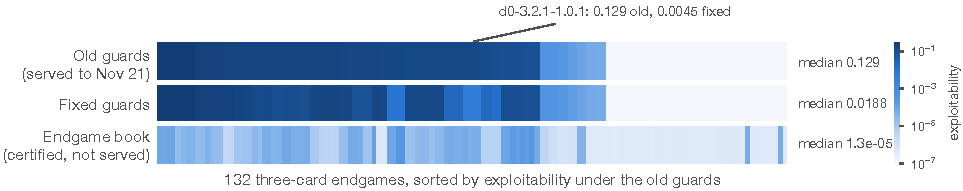
\includegraphics[width=\linewidth]{figures/fig_guards.pdf}
\caption{Each column is one three-card endgame, graded by \code{bin/bluff} at the class prior;
darker is more exploitable. The original guards made 24 more endgames exploitable by over $0.1$.
The belief reset leaves the dark block on the left, which the endgame book clears at the prior.}
\label{fig:guards}
\end{figure}

Each verdict comes with the best response that achieves it, which points straight at where a
strategy leaks. In the clearest case the bot holds two red cards. The opponent has one card left,
publicly known to be black, and bids ``one black''. That bid is true, so a challenge loses for
certain. The other moves are raises, such as ``two black'', which can't be true, since there is
only one black card in play. The guard deleted the raises as impossible and left the bot the
challenge, which always loses. But the opponent does not know the bot's cards, so a raise loses
only if the opponent calls it. So an impossible bid works as a bluff. The guard was written to stop the bot
from making false claims, and in a game about bluffing that meant it would never bluff when it was
cornered. In that class the guard took the bot from
$0.0045$ to $0.1286$. No meter inside the solver could have shown this bug. The guards ran after the solver was done,
so the solver measured the strategy it wrote and the site played a different one.

The fix forces a challenge only of a bid that is provably false, keeps a guard against flipping
into a certain loss, and prunes nothing else. I withdrew the paper's claim and replaced the guards
on the site. % NOAH-CONFIRM (first-person action)
% NOAH-CONFIRM (first-person action): the next sentence
With the fix I added an \emph{endgame book} for the same 168 classes, each computed as its own game
and certified by the checker (median exploitability $1.3\times10^{-5}$, worst
$3.05\times10^{-4}$). Each certificate holds only at the class prior, the belief about the opponent's
cards that the class starts from.

\section{A ceiling for the full game}\label{sec:whole}

Those 168 endgames are the part of Red/Black that fits in a file. The full game has about
$2.4\times10^{33}$ information sets \cite{rb1}. Over the summer I tried to prove an upper bound on
how exploitable the full-game bot is, and stopped with a lower bound only \cite{rb3}. % NOAH-CONFIRM (first-person action)
So for the bot as a whole I had the solver's word and a probe. Against the original bot, whose
meter read under $10^{-4}$ on every endgame I graded, the probe won $79.7\%$ of 6,000 games
($\varepsilon_G=1.19$).

For the full game the claim I wanted was a % NOAH-CONFIRM (states an intention)
ceiling, a number no opponent can exceed against the exact bytes the site serves. A ceiling is
computable when the bound is taken against an opponent stronger than any real one. The first policy
I could bound plays from the position class and its own \emph{type} alone (the reds in its hand and
among its discards). Suppose the opponent is told that type every time a round ends. Then nothing
carries across rounds, the best response is a dynamic program over classes, and the real opponent,
who is told nothing, can only do worse. The cost is that the bound charges the bot for a leak that
never happens.

\begin{figure}[t]
\centering
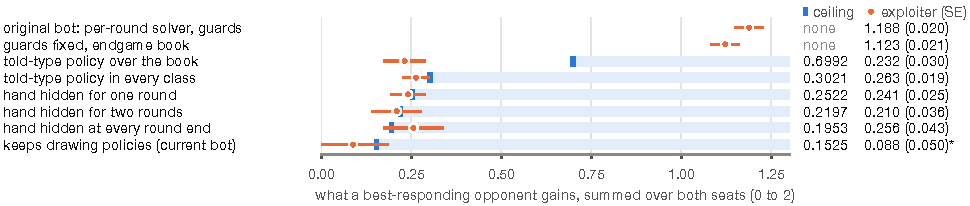
\includegraphics[width=\linewidth]{figures/fig_bound.pdf}
\caption{The stages of the site's bot, in order. Blue: the computed ceiling on what any
opponent can gain, $\varepsilon_G$ (the scale runs to 2). Orange: what the probe took, with
95\% intervals. The starred reading is interim (\servedprobepairs). The ceilings assume private
coins.}
\label{fig:bound}
\end{figure}

Figure~\ref{fig:bound} lists the stages. The told-type policy first ran above the endgame book,
and the ceiling for exactly that mix was $0.70$. The book was the weak part: it is exact at the
class prior and was never built to hold up against an opponent told its cards. With the told-type
policy in every class the ceiling was $0.302$. Everything after that came from one idea, which is
to stop telling the opponent the hand. At the end of a round the bot now privately draws one of
several stored policies for the next round, each built to play a whole range of its possible
hands. In the bound the opponent is told which policy was drawn and never the hand. The first
hidden-hand policy hides the hand this way through one round, and its ceiling was $0.2522$.
% SERVED-PROSE (1 of 3): the next two sentences name the current bot's stage and its numbers.
Hiding it through two rounds gave $0.2197$, and at every round end $0.1953$. The current bot, the one on
the site as of late November 2026, also keeps drawing fresh policies once the bound's opponent has
pinned down the hand, and its ceiling is $\servedbound$. No opponent can expect to win more than
$\servedwin$ of a seat-swapped pair of games against it. The same computation brackets the value
of the game for the first bidder between $\servedvlo$ and $\servedvhi$, where a win is $+1$. The
midpoint has sat near $+0.02$ at every stage, which I read as % NOAH-CONFIRM (his reading)
a small edge for whoever bids first, though nothing here proves it.

% SERVED-PROSE (2 of 3): this paragraph lists the checks run on the current bot's store.
These ceilings are 64-bit floating-point computations, so they are worth only the checks behind
them. A second implementation, written from the file format and the rules and sharing no code with
the solver, recomputed the bound from the served bytes, all 147,541 stored policies and both
opening positions, and agreed to within $10^{-15}$. With one layer's draws
into single-hand policies removed its bound rises to $0.2024$, so it does read that layer. \code{bin/bluff} graded the opening
round for both seats and 76 sampled stored policies in exact arithmetic on real one-round game
trees, and the largest disagreement was under $10^{-16}$. The site's
own TypeScript, replayed on 20,000 games and 0.9 million decisions, played the stored policy byte
for byte and never showed a client the draw. And the probe, rebuilt to track the draws, took
$0.2407$ (SE $0.025$) from the first hidden-hand policy and $\servedprobe$ (SE $\servedprobese$) so far from
the current one.

Every one of these ceilings also assumes the bot's coin flips are private, and on the live site
they were not. The server drew each bot move from a generator seeded with the game's id, a counter
and the seat, all of which a browser can see, and the generator is in the JavaScript the site sends to every browser. Anyone who ran that code could know
each coin before the bot flipped it, and against that opponent the bot was a pure strategy and no
number above applied. The solver, the bound computation, the second implementation and the probe all modeled
the coins as private, so none of them could see it. A replay of seven finished games from their
public records predicted all 103 of the bot's mixed decisions, where chance would get about
57. The coins now come from the secret seed that deals the cards, which no client sees until the
game ends, and the same replay does no better than chance (21 of 32, where chance is 18). Games
played before that change are outside every bound here.

\section{Limitations}

Everything above the endgames is floating point. The exact checker graded pieces of it, one round
at a time, but nothing is exact end to end. The told-type values under the hidden rounds exist in
three implementations that agree, which is evidence short of a proof. The ceiling covers
two-player games against the full-strength bot. It says nothing about three or more players or
about the site's weaker personas, which leave the stored policy on purpose.

The game files are
checked only against my own engine and rules document, so a misreading shared by both would pass.
The agent experiment has four replicates per model and setting, one prompt and small games whose values some
agents knew by heart.

The probe could not tell the first hidden-hand policy from the told-type policy.
On the same 3,000 deals it took $0.2407$ from the first and $0.2373$ from the second,
a difference well inside its standard error of $0.033$. Only for the current bot did its take
fall too, by $0.187$ (SE $0.076$) against the stage before it, over the first 525 deals of that run. One reading,
$0.256$ (SE $0.043$) for the stage that hides the hand at every round end, sits $1.4$ standard errors
above that stage's ceiling, which I report and cannot explain. On small classes where exact values
exist, about three quarters of what the ceiling charges is real and the rest is the told opponent.

% SERVED-PROSE (3 of 3): if a later store is served, rewrite this paragraph's first sentences.
A further pass over the stored policies computes a ceiling of $0.1432$. An independent
recomputation and a replay of the site's code agree with it, but its exact-tree samples and its
probe are not finished, so the site does not use it. The probe's noise is already larger than the
gap it is supposed to measure, so it should be replaced by a best response trained against the
bot's policy.

\section{Conclusion}

The hand in Section~\ref{sec:guards} is worth exactly a quarter, and the checker proves that for
the file I wrote. It proves a half for the leaky file just as readily, so the proof is only as good
as the match between the game file and the rules I meant, which I checked against the engine and
against nothing formal. For the full game the bot has a floating-point ceiling of $\servedbound$
and no exact certificate. That ceiling was computed from the bytes the site serves and recomputed
by a program that shares no code with the solver.

{\small\noindent\textbf{Acknowledgment.} AI tools helped me with parts of this project's
implementation, as the course allows.\par} % NOAH-CONFIRM (disclosure wording and whether the course wants it)

{\footnotesize
\bibliographystyle{abbrvnat}
\bibliography{refs}
}

\end{document}
